% !TeX spellcheck = en_GB
% !TeX root = ../phd-thesis.tex

\begin{figure*}[t]
    \centering
    \def\astscale{0.4}
    \begin{minipage}[c]{0.4\textwidth}
        \centering
        \begin{subfigure}{\linewidth}
            \centering
            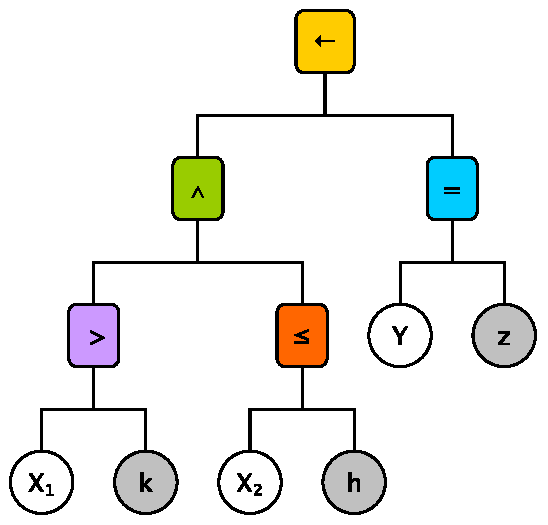
\includegraphics[scale=\astscale]{figures/ast-unencoded}
            \subcaption{AST of a logic formula}
            \label{fig:ast-kill-unencoded}
        \end{subfigure}
        \vspace{1.5ex}
        \tikz{\draw[->, thick] (0,0) -- (0,-0.4);}
        \vspace{2ex}
        \begin{subfigure}{\linewidth}
            \centering
            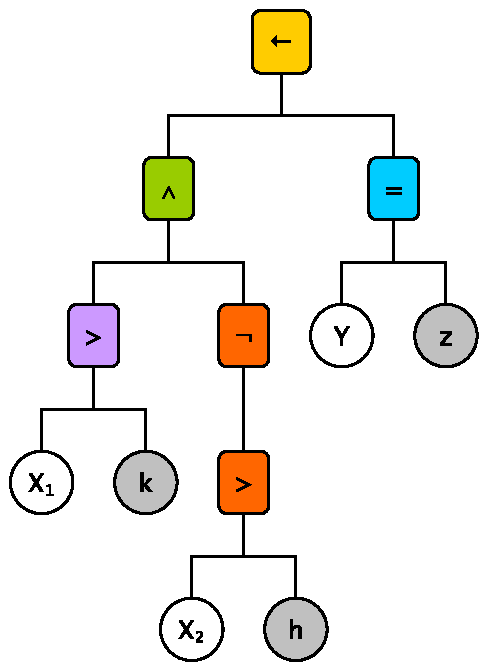
\includegraphics[scale=\astscale]{figures/ast-simplified}
            \subcaption{Simplified AST of a logic formula}
            \label{fig:ast-kill-simplified}
        \end{subfigure}
    \end{minipage}
    \hspace{0.5cm}
    \raisebox{-1cm}{\tikz{\draw[->, thick] (0,0) -- (0.7,0);}}
    \hspace{0.5cm}
    \begin{minipage}[c]{0.4\textwidth}
        \centering
        \begin{subfigure}{\linewidth}
            \centering
            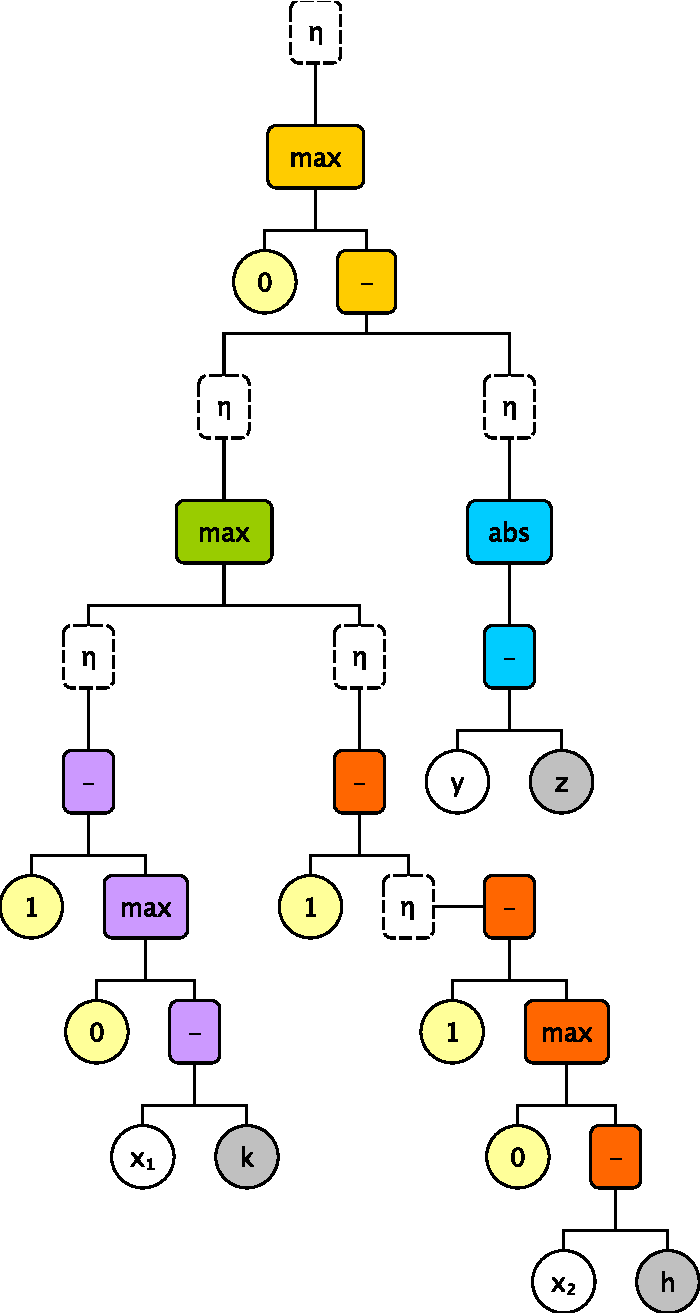
\includegraphics[scale=\astscale]{figures/ast-encoded}
            \subcaption{AST of the same formula, encoded as real-valued function}
            \label{fig:ast-kill-encoded}
        \end{subfigure}
    \end{minipage}
    \caption[KILL Encoding of logic formulas into real-valued functions]{
        %
        Example of the encoding process of logic formulas into real-valued functions.
        %
        Only \gls{AST} are depicted.
        %
        Boxes coloured in the same way represent the encoding of a given operator through each encoding step.
        %
        For instance, operator $<$ (red) is first converted into a negated $\geq$, and then into a combination of $max$ and subtractions.
    }
    \label{fig:ast-kill}
\end{figure*}
